% SPDX-FileCopyrightText: 2026 Will Cook
% SPDX-License-Identifier: CC-BY-4.0
\documentclass[11pt]{article}
% House typography (shared with the companion Lean papers): TeX Gyre Pagella
% under Tectonic/XeTeX, the same Palatino design through newpx under pdflatex.
\usepackage{iftex}
\ifpdftex
  \usepackage[T1]{fontenc}
  \usepackage[utf8]{inputenc}
  \usepackage{newpxtext}
  \usepackage{newpxmath}
\else
  \usepackage{fontspec}
  \usepackage{unicode-math}
  \setmainfont{texgyrepagella}[Extension=.otf,UprightFont=*-regular,
    BoldFont=*-bold,ItalicFont=*-italic,BoldItalicFont=*-bolditalic]
  \setmathfont{texgyrepagella-math.otf}
  \setmonofont{Inconsolatazi4}[Extension=.otf,UprightFont=*-Regular,
    BoldFont=*-Bold,Scale=MatchLowercase]
\fi
\usepackage[a4paper,textwidth=418pt,textheight=636pt,hcentering,
  top=68pt,headheight=15pt,headsep=20pt,footskip=34pt]{geometry}
\usepackage{booktabs,array,enumitem,microtype}
\linespread{1.045}
\clubpenalty=10000 \widowpenalty=10000 \tolerance=1600
\emergencystretch=2em
\usepackage[dvipsnames]{xcolor}
\definecolor{linkexternal}{HTML}{275D8C}
\definecolor{linkinternal}{HTML}{6E2B2B}
\usepackage[colorlinks=true,linkcolor=linkinternal,urlcolor=linkexternal,citecolor=linkinternal]{hyperref}
\usepackage{fancyvrb}
\usepackage{tikz}
\usetikzlibrary{positioning,arrows.meta,calc}
\usepackage{caption,float}
\captionsetup{font=small,labelfont=bf,skip=9pt,width=0.92\linewidth}
\fvset{fontsize=\small}
\setlist{nosep,leftmargin=*}
\setlength{\parindent}{0pt}
\setlength{\parskip}{0.55em}
\newcommand{\code}[1]{\texttt{#1}}
\newcommand{\component}[1]{\nolinkurl{#1}}
\newcommand{\repo}{\href{https://github.com/wcook04/plectis}{\nolinkurl{github.com/wcook04/plectis}}}

% Shared figure styles: black mechanism, dashed unavailable/unestablished
% material, and two accents used with one meaning each across all figures:
% blue for what a stranger can do, amber for words and choices the project
% itself supplies.
\colorlet{strangerblue}{RoyalBlue}
\colorlet{authoramber}{BurntOrange!85!black}
\tikzset{
  part/.style={draw=black!75, line width=0.6pt, rounded corners=2pt,
    align=center, inner sep=4pt, font=\footnotesize, fill=gray!8},
  words/.style={part, fill=white, draw=authoramber!75},
  ghost/.style={draw=black!45, dashed, line width=0.6pt, rounded corners=2pt,
    align=center, inner sep=4pt, font=\footnotesize, text=black!60, fill=none},
  act/.style={font=\scriptsize\itshape, text=strangerblue, align=center},
  gnote/.style={font=\scriptsize, text=black!60, align=center},
  flow/.style={-{Stealth[length=2.2mm]}, line width=0.6pt, draw=black!75},
  softflow/.style={-{Stealth[length=2.0mm]}, line width=0.6pt, draw=black!50, dashed},
  authlink/.style={softflow, draw=authoramber!70},
  actflow/.style={-{Stealth[length=2.0mm]}, line width=0.6pt, draw=strangerblue},
  flabel/.style={font=\scriptsize, inner sep=2pt},
  gaplabel/.style={font=\scriptsize, fill=white, inner sep=2.2pt, align=center,
    text=authoramber},
}

% These values are checked against the public registries by
% scripts/check_public_system_paper.py.  Do not update them from memory.
\newcommand{\snapshotcommit}{57ffb7f5830cc446a2cbd8083d5d80bcab2af563}
\newcommand{\snapshotshort}{57ffb7f5830c}
\newcommand{\componentcount}{88}
\newcommand{\familycount}{7}
\newcommand{\entrycount}{2}
\newcommand{\mappingcount}{12}
\newcommand{\mathcount}{20}
\newcommand{\safetycount}{20}
\newcommand{\researchcount}{9}
\newcommand{\publiccopycount}{20}
\newcommand{\recoverycount}{5}
\newcommand{\leanfilecount}{58}
\newcommand{\copiedsourcecount}{21}
\newcommand{\refactorcount}{27}
\newcommand{\runtimecount}{22}
\newcommand{\validatorcount}{18}

\hypersetup{
  bookmarksnumbered=true,bookmarksopen=true,bookmarksopenlevel=1,
  pdftitle={Plectis: What a Stranger Can Check},
  pdfauthor={Will Cook},
  pdfsubject={Public evidence from a private system: what a stranger can check, what the author can only report, and what remains unestablished},
  pdflang={en-GB},
  pdfkeywords={research software, claim verification, public evidence, reproducibility, software artifacts, agent-assisted development},
}
% Front-matter and sectional architecture (house style).
\usepackage{titlesec}
\titleformat{\section}{\Large\bfseries}{\thesection}{0.85em}{}
\titlespacing*{\section}{0pt}{2.4ex plus .8ex minus .3ex}{1.2ex plus .3ex}
\titleformat{\subsection}{\large\bfseries}{\thesubsection}{0.8em}{}
\titlespacing*{\subsection}{0pt}{1.9ex plus .6ex minus .2ex}{0.9ex plus .2ex}
\usepackage{fancyhdr}
\pagestyle{fancy}
\fancyhf{}
\fancyhead[L]{\small\itshape Plectis: what a stranger can check}
\fancyhead[R]{\small\thepage}
\renewcommand{\headrulewidth}{0pt}
\fancypagestyle{plain}{\fancyhf{}\renewcommand{\headrulewidth}{0pt}}
\renewcommand{\arraystretch}{1.12}

\makeatletter
\newcommand{\subtitle}[1]{\gdef\@papersubtitle{#1}}
\renewenvironment{abstract}{%
  \vspace{0.1em}\small
  \begin{center}{\normalsize\scshape Abstract}\end{center}\vspace{-0.5em}
  \list{}{\leftmargin 1.3em\rightmargin\leftmargin\listparindent 0pt
    \parsep 0.32em\itemindent 0pt}\item\relax}
  {\endlist\vspace{0.5em}}
\def\@maketitle{%
  \newpage\null
  \vspace*{-2.6em}%
  \begin{center}%
    {\LARGE\bfseries\@title\par}%
    \vskip 0.55em
    {\large\itshape\@papersubtitle\par}%
    \vskip 1.1em
    {\scshape\@author\par}%
    \vskip 0.25em
    {\small\@date\par}%
    \vskip 0.8em
    \rule{6.5em}{0.4pt}%
  \end{center}%
  \vskip 0.9em}
\makeatother

\title{Plectis: What a Stranger Can Check}
\subtitle{What public evidence can and cannot show about a private system}
\author{Will Cook}
\date{July 2026}

\begin{document}
\maketitle

\begin{abstract}
Plectis is a public software repository (an organised, copyable project
folder) built to expose selected claims about a larger private system. This
paper asks what a stranger may reasonably conclude from public tests when the
system stays private and its author chose both what to publish and what counts
as a pass. The answer is narrow. The repository lets a reader inspect and rerun
its published procedures, but a matching result cannot establish the hidden
system's history, whether the published selection resembles the private whole,
or whether the private system works reliably.

In the version studied here, each of the \componentcount{} registered components
(separately testable parts) connects a claim to a fixed input, command, saved
output, pass rule, and stated limit. I call this a claim--evidence--limit
contract. One component calculates an audio level from five small sample
arrays; a reader can repeat it and challenge the expected numbers. That run
still cannot show whether the pass rule tests the claim as written, how the
code behaves on untested inputs, or whether risks outside the declared scan are
absent. I chose the published fragments, inputs, answers, rules, and limits.
The repository therefore lets a reader test claims about its published files
and outputs, within those limits. I report that its published material was
copied or adapted from the private system, which remains unpublished because it
contains personal records, credentials, and unfinished tools. I also report
that I developed it by directing coding tools based on artificial intelligence
(AI). The argument does not depend on that account or on the claimed origin of
the published material.
\end{abstract}

\section{The problem}
\label{sec:problem}

I have a larger private software system that I cannot responsibly publish:
it contains personal records, credentials, live browser and account
information, my working notes, and unfinished tools. I would still like
strangers to be able to test some claims about it instead of accepting my
say-so. I use \emph{answerable} in a deliberately local sense. A claim is
answerable when a stranger can run a public procedure that bears on it, see
how the result is judged, and point a disagreement at a named public input,
rule, or output. This says nothing yet about whether the claim is true,
important, or representative of the hidden system. This paper asks what
conclusions that narrow form of answerability can support when the public
fragments come from a system no reader can see.

Plectis is my working answer: a public software repository, stored at
\repo. A \emph{repository} is an organised project folder, usually kept
with its revision history; to \emph{clone} a repository is to copy that
folder and history to another computer. Everything this paper says a
stranger can check is in that repository. This paper describes how its
claims are exposed and where the evidence stops.

I am 22 and study economics. Over about ten months I built the private
system by directing AI coding agents, software tools that can edit, run, and
revise code across a task. I set objectives and review criteria,
accepted or rejected their output, and sent them back to revise failures;
the agents wrote nearly all of the code, and I wrote nearly none of it. No
other person worked on the system. This account explains why the publication
problem arose and why the choices examined below are my responsibility, but
it remains testimony about origin. Plectis can expose public files and runs;
it cannot independently prove how the private work was produced. The
public repository does not prove the story, and the argument does not rely on it.

The limit on what a public run can establish would be the same if every line
had been written by hand. Authorship might affect how often a failure occurs:
for example, an implementation and the program that checks it can share a mistake when
one process drafts both. This paper compares no development methods and
estimates no error rates.

The boundary of the evidence can be stated before any command is run:

\begin{center}
\small
\begin{tabular}{>{\raggedright\arraybackslash}p{0.24\linewidth}>{\raggedright\arraybackslash}p{0.67\linewidth}}
\toprule
\textbf{Status} & \textbf{What belongs in it} \\
\midrule
Publicly checkable & The contents of a named public version, the commands listed for its components, the files those commands write, and the results of its public tests. \\
Reported here & The private system's history, the role of AI agents in producing it, and my claim that the published material came from the private system. \\
Not established here & Whether the public selection represents the private whole, whether the published code works beyond its fixed inputs, whether the project's own pass rules are correct or even test the stated claims, and whether the private system works reliably at all. \\
\bottomrule
\end{tabular}
\end{center}

\paragraph{What I examined.} The paper examines one author-curated software
collection. At the named repository version, I read the list
and plain descriptions of all \componentcount{} components, counted them by
project group and by the kind of public evidence offered, traced the worked
component from input to limit, and reran the appendix's public commands. I did
not compare every pass rule with its prose claim or derive fresh expected
answers; Section~\ref{sec:stronger} reserves those checks for an outside
evaluator. The paper defines the component contract, then follows
one ordinary component from input to limit. Five distinctions separate what a
passing run shows from conclusions it may appear to support. The final
sections identify the choices an evaluator would need to make independently
of me.

This is a descriptive analysis of one public repository, not a statistical
study. Runeson and H\"ost distinguish a case from the units of analysis within
it \cite[\S2.5]{runeson2009}. I borrow only those two terms: the named repository
version is the single case, and each component is a \emph{unit of analysis}
(one item examined inside that case). This paper does not otherwise claim a
full case-study design. No subset of the components is used to estimate
performance or represent the private system.

Reading this paper requires no programming. Reproducing its runs requires
basic command-line use, a terminal (a text window for commands), Git (for
copying and versioning repositories), Python 3.11 or later, and \code{pip}
(for installing Python software). The appendix gives the exact commands,
environment details, and installation notes. It is a dated record of one
verification pass at the version named there.

\section{The component contract}
\label{sec:contract}

A \emph{component} in Plectis is one registered, testable part of the
project. Its \emph{fixture} is a fixed sample input. A \emph{receipt} is the
saved record of a run. The repository supplies one from an earlier run;
rerunning can write another. A \emph{validator} is the program that applies a
component's pass and refusal rules. A
\emph{commit} is a named, saved version of the repository. These terms
describe files and commands. Here \emph{evidence} means the public input,
procedure, output, and judgement rule offered in support of a claim. Calling
them evidence does not establish their adequacy. \emph{Contract} means only
that the claim, those materials, and a limit are stated together so readers
can check their fit. Nothing in these labels grades the importance of what a
component does.

At commit \code{\snapshotshort} the registry, the component list read by the
programs, contains \componentcount{} entries. Every entry is required to
connect the same things: a claim stated in prose; a fixture; a command; the
output files the command writes; a stored receipt from a prior run; an
explicit rule for what counts as a pass and what must be refused; and a
stated limit on what a pass establishes. Figure~\ref{fig:contract} lays the
required parts out, together with the fact about them that the rest of this
paper keeps returning to: every part is supplied by me, and every part is
exposed to a stranger.

\begin{figure}[t]
\centering
\makebox[\linewidth][c]{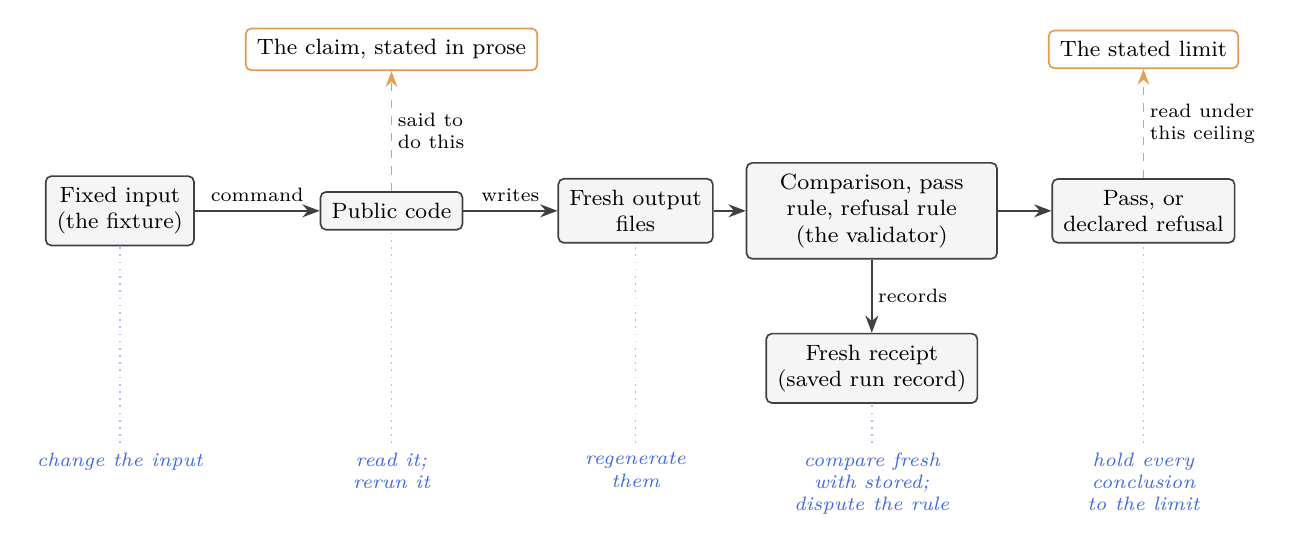
\begin{tikzpicture}[x=1cm,y=1cm]
% words row
\node[words] (claim) at (3.45,2.05) {The claim, stated in prose};
\node[words] (limit) at (13.0,2.05) {The stated limit};
% mechanism row
\node[part] (fix) at (0,0) {Fixed input\\(the fixture)};
\node[part] (code) at (3.45,0) {Public code};
\node[part] (out) at (6.55,0) {Fresh output\\files};
\node[part, text width=2.9cm] (val) at (9.55,0) {Comparison, pass rule, refusal rule\\(the validator)};
\node[part] (verdict) at (13.0,0) {Pass, or\\declared refusal};
\node[part] (rec) at (9.55,-2.0) {Fresh receipt\\(saved run record)};
% flows
\draw[flow] (fix) -- node[flabel, above=1pt]{command} (code);
\draw[flow] (code) -- node[flabel, above=1pt]{writes} (out);
\draw[flow] (out) -- (val);
\draw[flow] (val) -- (verdict);
\draw[flow] (val) -- node[flabel, right]{records} (rec);
\draw[authlink] (code) -- node[flabel, right, align=left]{said to\\do this} (claim);
\draw[authlink] (verdict) -- node[flabel, right, align=left]{read under\\this ceiling} (limit);
% stranger actions
% top-anchored so the action row reads as one aligned row despite
% differing line counts
\node[act, anchor=north] (a1) at (0,-2.95) {change the input};
\node[act, anchor=north] (a2) at (3.45,-2.95) {read it;\\rerun it};
\node[act, anchor=north] (a3) at (6.55,-2.95) {regenerate\\them};
\node[act, anchor=north] (a4) at (9.55,-2.95) {compare fresh\\with stored;\\dispute the rule};
\node[act, anchor=north] (a5) at (13.0,-2.95) {hold every\\conclusion\\to the limit};
\draw[RoyalBlue!45, dotted, line width=0.6pt] (a1) -- (fix);
\draw[RoyalBlue!45, dotted, line width=0.6pt] (a2) -- (code);
\draw[RoyalBlue!45, dotted, line width=0.6pt] (a3) -- (out);
\draw[RoyalBlue!45, dotted, line width=0.6pt] (a4) -- (rec);
\draw[RoyalBlue!45, dotted, line width=0.6pt] (a5) -- (verdict);
\end{tikzpicture}}
\caption{How to read the component contract, at commit
\code{\snapshotshort}. Read the middle row from left to right: a command applies
public code to a fixed input and the code writes output. The validator judges it
under the published pass and refusal rules, then writes a fresh receipt recording
the run. The stored receipt from the earlier run is available for comparison; it
does not determine the new verdict. The two
boxes above are words rather than mechanisms: the project states the claim and
the limit on what a pass may support. Every part is public, and the project
supplied every part. The italic blue row names what a stranger can do without
asking anyone; amber marks the project's words and choices. Across the figures,
a dashed outline marks something outside what the public run establishes. This
figure has no dashed boxes because none of its parts is hidden. In
Figures~\ref{fig:boundary} and~\ref{fig:gaps}, dashes mark private material or
conclusions not established by the observed run. Section~\ref{sec:run} follows
one component through this chain.}
\label{fig:contract}
\end{figure}

The repository cannot by itself support my assertions about the unseen private
system. A component does something narrower: it gives a related public claim a
procedure that can fail in front of a stranger. The procedure
does not make the claim true or establish the published fragment's origin. It
changes the form disagreement can take: a reader who doubts a component's
claim can point at a particular input, a particular line of the validator, or a
particular number in the output, instead of arguing with my description of
software they cannot see. A component that fails is still answerable in
this sense, and a component can be answerable and trivial; answerability
concerns the form a claim takes, not its truth and not its importance.

A component may also end in a declared refusal rather than an answer. The
worked example below refuses an input format it does not support. Components
that depend on an external tool, such as the Lean proof checker (a program
that verifies mathematical proofs), must record a refusal with a stated limit
when the tool is absent, rather than reporting success.
\emph{Runnable} therefore means that the operation and its declared failure
boundary are present in public form; it does not mean that every optional
dependency exists on every machine. A refusal is informative only when it is
declared in advance and distinguishable from a breakdown: a predeclared
refusal marks the edge of what the component claims, while an unexpected
crash is a defect. The two must not be read as the same kind of event. One
honesty condition on refusals cannot be discharged from inside the
repository at all: the public record shows each boundary as declared at the
named commit, and it cannot show whether the boundary was drawn before or
after an awkward case was first met. A boundary drawn afterwards turns a
failure into a designed refusal in the telling. Saving the version before
an outside evaluation begins, as Section~\ref{sec:stronger} proposes, is
what would make that ordering checkable.

The idea does not depend on software. The contract needs a claim in words; a
determinate public case; a procedure a stranger can
cause to run; an observable result; a rule connecting result to claim; a
declared boundary of application; and a stated ceiling on inference. That
the case here is a file of numbers, the procedure a command, and the record a
text file is a convenience of this example. The same contract could be
satisfied in another field by a laboratory protocol with declared rejection
conditions, or by a sealed evaluation service with published scoring rules.
I make no claim about those settings; the point is only that the contract
is a shape for exposing claims to strangers, and this repository is one
example. Read simply as software, it is a test suite with a registry and
unusually complete paperwork. That is a fair description. The paper asks
what such a test suite lets a stranger challenge, and which conclusions
still lie beyond it.

This local notion overlaps with reproducibility and transparency but is not
a synonym for either. A run can repeat perfectly with no stated claim attached,
and a claim can be answerable while still awaiting a good test. The design
also begins from partial disclosure: it offers one limited point of contact,
not a view of the hidden system. A component exposes the published fragment
to challenge. It does not make the private whole answerable.

Answerability is not the same property as computational reproducibility,
although the component contract supplies materials needed to test the
latter. Under the convention used by the National Academies, computational
reproducibility means obtaining consistent results using the same input
data, computational steps, methods, code, and conditions of analysis; such
consistency does not by itself establish correctness
\cite[conclusion 3-1]{nasem2019}.
In software testing, a \emph{test oracle} is the information or procedure used
to decide whether an observed output is correct. The challenge of making that
distinction is called the test oracle problem \cite[p. 507]{barr2015}. The risk
that a curated collection disproportionately exposes favourable cases is
analogous to selective publication and the file-drawer problem
\cite{rosenthal1979}.
An \emph{assurance case} links a system claim to reasons and evidence. The
Object Management Group's Structured Assurance Case Metamodel (SACM), version
2.3, describes such cases as auditable claims, arguments, and evidence. Section
2.2 says the Claims--Arguments--Evidence notation has its own mapping onto SACM;
informative Annex A.2 points to the maintained mapping details
\cite[secs. 1.1, 2.2; Annex A.2]{omgsacm2023}. Plectis is
not an implementation of that standard and makes no claim that the private
system is safe. Its validator applies a published rule; it does not supply the
full argument from evidence to claim that an assurance case would require.
The Association for Computing Machinery (ACM) calls digital research materials
such as code, scripts, and data
\emph{artifacts}. Its \emph{Artifacts Evaluated---Functional} badge means
those materials passed an independent audit for documentation, consistency,
completeness, ability to run, and evidence of verification and validation.
\emph{Results Reproduced} means another team later obtained the main results
using some author-supplied artifacts \cite{acmartifact}. Plectis claims neither
status. These standards are comparison points, not statuses awarded here. This
paper claims no new theory of assurance, testing, or reproducibility; it reads
each public procedure against its claim and stated limit.

\section{One run, examined}
\label{sec:run}

The component \component{batch8_audio_level_rms_port} computes a loudness
level from short arrays of audio samples. I chose it because it is ordinary.
It needs only a square root and no knowledge of the private system; its claim
is small enough that every part of the evidence can be seen at once.

The reported origin is this. The private system contains a small macOS
recording application, and one of that application's functions reduces a
short stretch of audio samples held in memory to a level between zero and
one. The public
component re-expresses that calculation in Python. The component's code and
its stored receipts name the private file it claims to re-express
(\component{AudioLevelMonitor.swift}); a stranger cannot open that file, so
the name is a report, not evidence. What the stranger can check is
everything else.

The declared calculation begins with root-mean-square (the \code{rms} in
the component's name): square each sample, average the squares, and take
the square root. It then applies the project's gain of eight and caps the
result at one. Signed sixteen-bit integer samples are first divided by
32{,}767, the largest positive value in that representation, to bring them
onto the same scale. An empty input must produce zero. An unrecognised
format name must be refused rather than guessed at.

The component's public command runs it against its fixture and writes fresh
output outside the repository (the backslashes split one long command across
lines):

\begin{Verbatim}[fontsize=\small]
PYTHONPATH=src python3 -m plectis \
  batch8-audio-level-rms-port run \
  --input fixtures/first_wave/batch8_audio_level_rms_port/input \
  --out /tmp/plectis-audio-rms \
  --acceptance-out /tmp/plectis-audio-rms-acceptance.json
\end{Verbatim}

At commit \code{\snapshotshort}, the run produced:

\begin{center}
\small
\begin{tabular}{>{\raggedright\arraybackslash}p{0.21\linewidth}>{\raggedright\arraybackslash}p{0.26\linewidth}>{\raggedleft\arraybackslash}p{0.15\linewidth}>{\raggedleft\arraybackslash}p{0.15\linewidth}>{\raggedright\arraybackslash}p{0.09\linewidth}}
\toprule
\textbf{Case} & \textbf{Input} & \textbf{Expected} & \textbf{Observed} & \textbf{Result} \\
\midrule
Decimal samples & 0.0,\ 0.05,\ $-0.05$,\ 0.1 & 0.489897949 & 0.489897949 & pass \\
Sixteen-bit integer samples & 0,\ 1638,\ $-1638$,\ 3277 & 0.489892970 & 0.489892970 & pass \\
Values above the cap & 1.0,\ $-1.0$,\ 0.5 & 1.000000000 & 1.000000000 & pass \\
Empty input & (none) & 0 & 0 & pass \\
Unknown format & \code{pcm24} & refusal & refusal & pass \\
\bottomrule
\end{tabular}
\end{center}

Here \emph{pass} means ``refused as expected''; \code{pcm24} was not accepted.
Because the inputs and the rule are both printed above, the first row can be
checked without the repository or a computer: the squares of the four
samples average to 0.00375, whose square root is $0.061237\ldots$, and eight
times that is $0.489897\ldots$. A reader with a calculator can recompute this
expected value from the stated formula alone. For this one case the reader
can supply the test oracle: elementary arithmetic gives an expected number
derived independently of the program's output, but not of the project's
formula.

Almost nothing else in the collection is like that, which is why the example
matters. Elsewhere the project usually supplies the implementation, the
input, the expected values, and the validator through the same
author-controlled process. A test
assembled that way can pass for four different reasons: the implementation
and the expectation are both correct; the two share a mistake; the chosen
cases happen to sit where the implementation behaves; or the validator
checks a weaker property than the prose claim suggests. A matching result
therefore establishes repeatability under that public test. Independent
evidence bearing on correctness needs an expected result justified apart from
the implementation. Arithmetic supplies that for the first row only after
accepting the project's formula. Fresh inputs alone do not supply one.

The example suggests a question for any software test: where did the expected
value come from, and who supplied it? The answer changes what a match can
support:

\begin{center}
\small
\begin{tabular}{>{\raggedright\arraybackslash}p{0.44\linewidth}>{\raggedright\arraybackslash}p{0.47\linewidth}}
\toprule
\textbf{Who or what supplies the expected answer} & \textbf{What a matching result then supports} \\
\midrule
The project itself: implementation, cases, expectations, and rule from one author-controlled process. & Repeatability under the project's own test; the four readings above all stay open. \\
\addlinespace
The reader derives a result from stated premises, as in the decimal-samples row. & Agreement with the stated formula on that case, not proof that the formula is right. \\
\addlinespace
An established external tool or reference. & Whatever the reference itself warrants, on the cases run, within the reference's own limits. \\
\addlinespace
An evaluator who chooses inputs and independently justifies expected results after the version is saved. & Independent evidence bearing on correctness for those cases, within the oracle's own justification and limits. \\
\addlinespace
The world: an outcome observed apart from any program. & Evidence about a real-world outcome, where one exists. \\
\bottomrule
\end{tabular}
\end{center}

Most components in the collection sit in the first position, except where
a reader promotes a case to the second by recomputing it, as the worked
example's decimal-samples row invites. Components that invoke a named
external tool occupy a hybrid of the first and third positions: the project
still chooses the case and the rule, while the tool supplies a result that
inherits its own limits. The evaluations in Section~\ref{sec:stronger} describe
ways to move consequential choices out of the project's control.

\component{batch8_audio_level_rms_port_validation_receipt.json} is the stored
reference for the table. It sits under
\component{receipts/first_wave/batch8_audio_level_rms_port/}, so a fresh run is
compared against a fixed record rather than against memory. A stored record by
itself does not prove that the stated command produced it; its use is that
anyone can generate a fresh one and compare the two.

The limit is part of the component. This run checks one public Python
calculation over synthetic sample arrays (arrays composed for the test, not
captured from a device). It does not run the original application, start an
audio session, request microphone permission, or capture sound, and it
cannot establish that the named private file is where the calculation came
from. Nor does the table show that the task was difficult (it was not),
that the component is useful elsewhere, or that the remaining entries
resemble it. What it shows is that one assertion now has a form in which a
stranger can rerun it, dispute its rule, perturb its input, or replace my
expected value with a better-derived one.

The calculator check derives one expected number without the implementation.
It shows agreement with the project-supplied formula on that case, not that
the formula is the right audio rule. It does not establish origin, reach, or
risks beyond the declared scans. Its correctness evidence is limited to that
calculation. The next section treats these five gaps separately.

\section{Five distinctions}
\label{sec:distinctions}

Five labels organise the gaps in Figure~\ref{fig:gaps}: \emph{origin}, where
the material came from; \emph{correctness}, whether an answer is right;
\emph{meaning}, whether a rule tests its claim; \emph{reach}, whether shown
cases stand for unshown ones; and \emph{risk}, what the declared checks may
miss. Each subsection separates observation from inference.

\subsection*{Public execution versus where the code came from}

A reader can establish what a named public commit contains and what its
commands do. No public run establishes where the material came from.
Plectis records that boundary. Each copied file has a claimed source and a
SHA-256 fingerprint: a fixed 256-bit value calculated from its contents and
used to detect change \cite{nistfips1804}. Two different files can in principle
have the same fingerprint. For this comparison, the relevant question is
whether one can start with a specified file and find a different file with the
same fingerprint. The National Institute of Standards and Technology (NIST)
calls this second-preimage resistance and expects an approved hash function to
make such a search computationally infeasible. That differs from collision
resistance, which asks only for any pair of different inputs that match
\cite[security-strength table]{nisthashfunctions}. A match therefore supports a
narrow claim: the public file's contents agree with the version represented in
its public record. But I control both sides, so that agreement is evidence of
internal consistency, not of origin. The same holds for the
audio component's named source file: the name is an entry I wrote. Origin
claims could only be strengthened by something a public repository cannot
supply about itself, such as commitments published before the fact, or a
trusted person permitted to examine both sides. The term \emph{provenance}
means an object's origin and history. Here, that origin remains reported
rather than publicly established.

\subsection*{Repeatability versus correctness}

A run that yields the same checked values and verdict as the stored receipt
shows that the public code, on the supplied input, in a sufficiently similar
environment, produces the same result again. Correctness is a different
property: it needs a standard for
what the result should have been, and a standard is only worth something if
it does not merely restate the implementation. The worked example makes the
difference concrete. The first row's expected number comes from arithmetic
applied to the project's formula, not from the implementation. That supports
agreement with the formula on one case; it does not validate the formula.
Most components have only the project's own expected values and validator.
Passing tests anywhere in Plectis should be read at that strength and no more.

\subsection*{A validator's rule versus the stated claim}

A pass is a verdict from the validator, and a validator checks exactly the
property written into it, which can be narrower than the claim as worded. A
component whose prose speaks of handling a class of inputs may in fact
verify that one output file exists and matches a stored shape; a rule can
hold while the sentence it stands under goes untested. The two previous
distinctions do not cover this gap: a result can be repeatable, and correct
as far as the checked property goes, while the checked property is beside
the stated point. Plectis makes the gap inspectable rather than closed.
Every validator is public, so a reader can put the rule beside the prose
and object where the rule is weaker, and the review in
Section~\ref{sec:conclusion} makes exactly that comparison its central step.
Since the same author-controlled project produced both the claims and the
rules, agreement between them records one judgement twice, and no count of
passing components can substitute for reading one rule against one sentence.

\subsection*{Selected cases versus general behaviour}

Selection acts at two levels. Within a component, the fixture covers only a
few possible inputs. Across the collection, the published components are my
selection from a private whole.

\begin{samepage}
I chose which mechanisms
could be given public form, which inputs to include, which expected values to
store, and which pass rules to enforce. Nothing in the public record shows
how many candidates there were, what was excluded beyond the privacy rules,
or whether the collection resembles ordinary work in the private system. A
collection can consist entirely of genuine items and still give an
unrepresentative picture of what it was drawn from. This is analogous to
selective publication and the file-drawer problem, not the same process
\cite{rosenthal1979}.
Figure~\ref{fig:boundary} draws the situation: public checking reaches
everything to the right of the boundary, and the pool the selection was
drawn from stays on the left.
\end{samepage}

\begin{figure}[H]
\centering
\makebox[\linewidth][c]{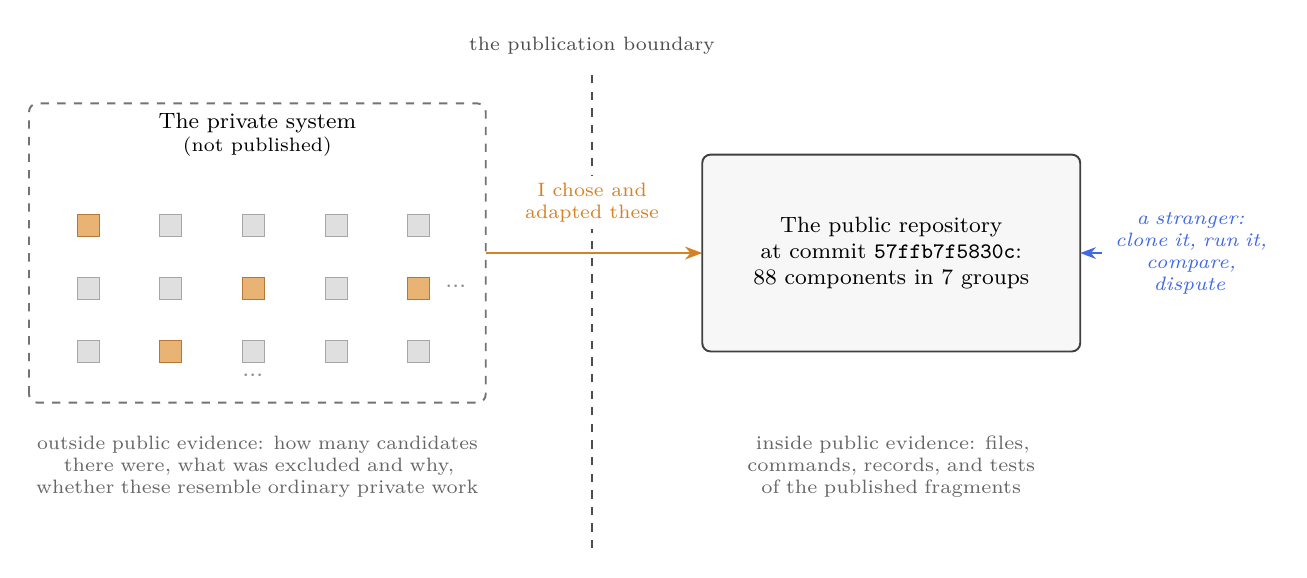
\begin{tikzpicture}[x=1cm,y=1cm]
% private region
\draw[black!55, dashed, line width=0.7pt, rounded corners=3pt] (0,-0.1) rectangle (5.8,3.7);
\node[font=\footnotesize, align=center] at (2.9,3.3) {The private system\\[-1pt]{\scriptsize (not published)}};
% mechanism squares: 5 x 3 grid, four of them selected (darker)
\foreach \x in {0.75,1.80,2.85,3.90,4.95}
  \foreach \y in {0.55,1.35,2.15}
    \draw[black!35, fill=gray!25] (\x-0.14,\y-0.14) rectangle (\x+0.14,\y+0.14);
\foreach \sx/\sy in {1.80/0.55,2.85/1.35,0.75/2.15,4.95/1.35}
  \draw[authoramber!80!black, fill=authoramber!55] (\sx-0.14,\sy-0.14) rectangle (\sx+0.14,\sy+0.14);
\node[font=\small, text=black!45] at (5.42,1.35) {$\cdots$};
\node[font=\small, text=black!45] at (2.85,0.22) {$\cdots$};
% boundary
\draw[black!70, dashed, line width=0.8pt] (7.15,-1.95) -- (7.15,4.15);
\node[font=\scriptsize, text=black!70, above] at (7.15,4.2) {the publication boundary};
% selection arrow; the label plaque interrupts the boundary line symmetrically
\draw[flow, draw=authoramber] (5.8,1.8) -- (8.55,1.8);
\node[flabel, fill=white, align=center, inner sep=2.5pt, text=authoramber] at (7.15,2.44) {I chose and\\adapted these};
% public box
\draw[black!75, line width=0.7pt, rounded corners=3pt, fill=gray!6] (8.55,0.55) rectangle (13.35,3.05);
\node[font=\footnotesize, align=center] at (10.95,1.8) {The public repository\\at commit \code{\snapshotshort}:\\\componentcount{} components in \familycount{} groups};
% stranger
\node[act, text width=2.0cm] (str) at (14.75,1.8) {a stranger:\\clone it, run it,\\compare, dispute};
\draw[actflow] (str.west) -- (13.35,1.8);
% notes
\node[gnote, text width=5.6cm, anchor=north] at (2.9,-0.40) {outside public evidence: how many candidates there were, what was excluded and why, whether these resemble ordinary private work};
\node[gnote, text width=4.6cm, anchor=north] at (10.95,-0.40) {inside public evidence: files, commands, records, and tests of the published fragments};
\end{tikzpicture}}
\caption{The selection problem. Each square stands for a private
mechanism; the darker ones were given public form. Each public component
has the parts shown in Figure~\ref{fig:contract}. The grid trails off
because its true extent is exactly what the public side cannot know. The
count of squares on the left, the
rule that picked the darker ones, and the resemblance between the two sides
are all invisible from the right. The collection supplies directly
checkable evidence about the published files and their behaviour under
named tests, but no basis by itself for generalising to the hidden whole.}
\label{fig:boundary}
\end{figure}

The registry's count should be read in that light. A registry of
\componentcount{} entries defines exactly what is published. A later
evaluation would need that list to draw a sample and report failure rates
against a fixed total. The count is an inventory, not a score, and
even the unit of counting is a choice I control, since one mechanism could
have been registered as several components, or several as one.

\subsection*{Risk reduction versus guarantee}

The publication process runs checks whose honest description is that they
reduce specific risks. Automated scans search copied material for specified
patterns of credentials, personal information, and private file paths, and
record what was omitted or rejected; a scan establishes that the scanner
did not find the patterns it was designed to find, and nothing stronger.
Pages such as the component map are generated from the registry, and tests
compare page and registry, which prevents the particular failure of prose
drifting away from records; a generator and its records can still be wrong
together. The documented \code{tour} run takes the public checkout as its
explicit input and does not automatically discover a neighbouring private
repository. The release-export contamination check is an explicit
exception: when a copy of the private project folder is available, it may
compare the contents of public source files with private files to detect
leakage. None of this
amounts to a guarantee that no secret, no identifying detail, and no
inconsistency survives. Publication remains a judgement about acceptable
risk, and I made it.

Origin evidence and privacy pull in opposite directions. Establishing
provenance would require someone to examine private
material, and the privacy constraint that motivates the whole design forbids
exactly that examination in public. Some claims are therefore permanently in
the reported category, short of a confidential review. The honest treatment
is to label them, not to dress them up as public proof through bookkeeping
that one maintainer controls.

\medskip

The same mistake lies behind all five: treating an observation as if it proved
something never tested. A broader conclusion needs an added assumption. For
origin, one must assume
that the public object came from the private one. For correctness, one must
know that the expected answer was right; for meaning, that the rule tested
what the claim said. For reach, one must assume that the chosen cases stand
for the unchosen; for risk, that the scan covered the relevant risks. The
observation itself supplies none of these assumptions. The contract makes
each one explicit. Once named, a gap can be disputed, assigned a cost to
address, or deliberately left open. An unnamed gap is easy to cross without
noticing. These five are not exhaustive. Two more gaps appeared earlier:
observing a refusal today does not show when it was drawn
(Section~\ref{sec:contract}), and observing a number at one commit does not
describe the next (the appendix). These are simply the five gaps this
collection most needs a reader to hold.

\begin{figure}[t]
\centering
\makebox[\linewidth][c]{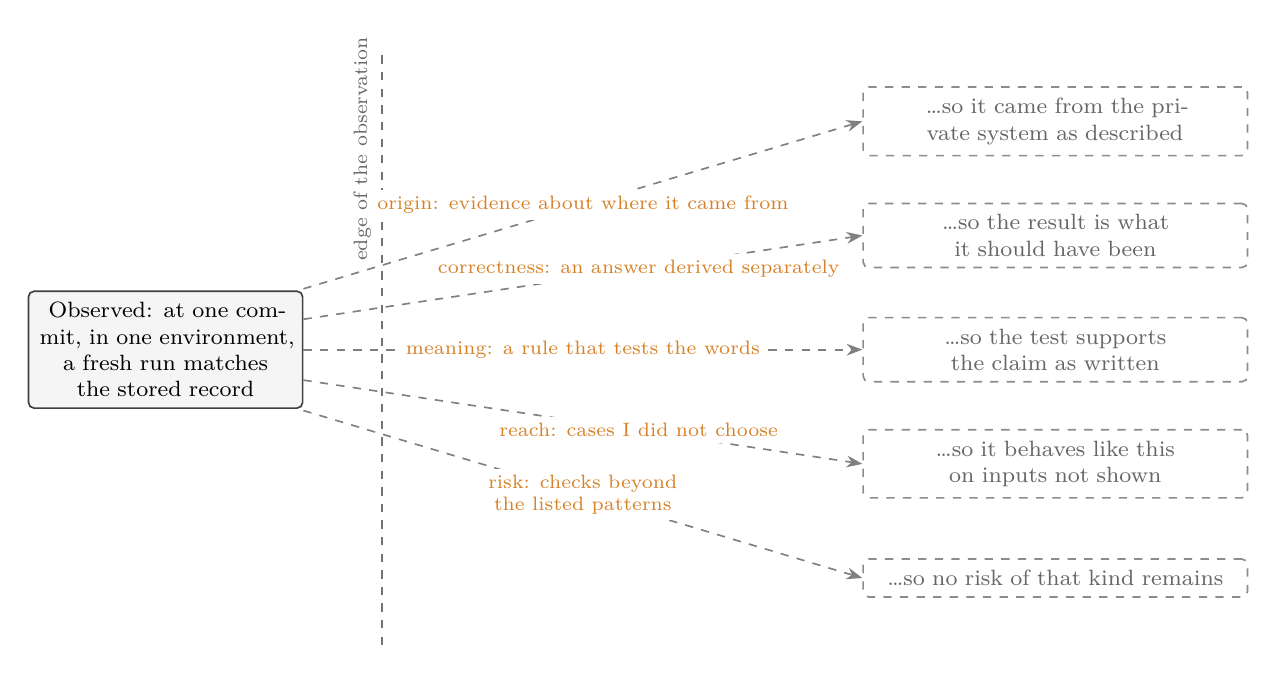
\begin{tikzpicture}[x=1cm,y=1cm]
\node[part, text width=3.2cm] (obs) at (1.8,0) {Observed: at one commit, in one environment, a fresh run matches the stored record};
\draw[black!55, dashed, line width=0.7pt] (4.55,-3.75) -- (4.55,3.75);
\node[font=\scriptsize, text=black!60, rotate=90] at (4.3,2.55) {edge of the observation};
\node[ghost, text width=4.6cm] (g1) at (13.1,2.9)  {\ldots so it came from the private system as described};
\node[ghost, text width=4.6cm] (g2) at (13.1,1.45) {\ldots so the result is what it should have been};
\node[ghost, text width=4.6cm] (g3) at (13.1,0)    {\ldots so the test supports the claim as written};
\node[ghost, text width=4.6cm] (g4) at (13.1,-1.45){\ldots so it behaves like this on inputs not shown};
\node[ghost, text width=4.6cm] (g5) at (13.1,-2.9) {\ldots so no risk of that kind remains};
% fanned starts so the five tails do not pile on one point; all lines are
% drawn first, then all label plaques, so no later line strikes a label
\draw[softflow] ([yshift=22pt]obs.east) -- (g1.west);
\draw[softflow] ([yshift=11pt]obs.east) -- (g2.west);
\draw[softflow] (obs.east) -- (g3.west);
\draw[softflow] ([yshift=-11pt]obs.east) -- (g4.west);
\draw[softflow] ([yshift=-22pt]obs.east) -- (g5.west);
\path ([yshift=22pt]obs.east) -- (g1.west) node[gaplabel, pos=0.50]{origin: evidence about where it came from};
\path ([yshift=11pt]obs.east) -- (g2.west) node[gaplabel, pos=0.60]{correctness: an answer derived separately};
\path (obs.east) -- (g3.west) node[gaplabel, pos=0.50]{meaning: a rule that tests the words};
\path ([yshift=-11pt]obs.east) -- (g4.west) node[gaplabel, pos=0.60]{reach: cases I did not choose};
\path ([yshift=-22pt]obs.east) -- (g5.west) node[gaplabel, pos=0.50]{risk: checks beyond\\the listed patterns};
\end{tikzpicture}}
\caption{Five conclusions a matching run invites and does not license.
Each dashed arrow needs a further assumption that the observation itself
cannot supply. From top to bottom, the tags follow the order discussed above:
origin (provenance), correctness, meaning, reach, and risk. The contract's
contribution is not to cross these gaps but to make them nameable, one
component at a time.}
\label{fig:gaps}
\end{figure}

\section{What the collection contains}
\label{sec:collection}

At commit \code{\snapshotshort} the \componentcount{} components fall into
\familycount{} groups:

\begin{center}
\small
\begin{tabular}{>{\raggedright\arraybackslash}p{0.38\linewidth}r>{\raggedright\arraybackslash}p{0.47\linewidth}}
\toprule
\textbf{Group} & \textbf{Count} & \textbf{What its components do} \\
\midrule
Getting started & \entrycount & Show a new reader where to begin and guide a first inspection. \\
Project mapping & \mappingcount & Map files and written rules, find relevant material, and route a question to the part of the project that owns it. \\
Computer-checked mathematics & \mathcount & Check records and fixed examples from formal mathematics, including small Lean statements and one exact finite calculation. \\
AI reliability and safety tests & \safetycount & Replay fixed cases involving hostile instructions, software boundaries, stored information, tool use, and benchmark rules. \\
Research-method tests & \researchcount & Exercise fixed cases involving replication, conflicting forecasts, explaining model behaviour, simulation, and laboratory safety. \\
Public-copy maintenance & \publiccopycount & Check copied source, generated pages, publication boundaries, and disagreement between records and derived files. \\
Work recovery & \recoverycount & Record unfinished changes and test how work resumes after interruption. \\
\bottomrule
\end{tabular}
\end{center}

The groups do not share a subject; computer-checked mathematics has nothing
in particular to do with audio levels or with recovering interrupted work.
Their unity is the contract of Section~\ref{sec:contract}: these are the
places in the private system where a mechanism could be turned into a small,
runnable public procedure. The collection is organised by how its claims are
checked, not by subject.

The registry also classifies what kind of evidence each component supplies.
It calls this classification a \emph{route}. A route says whether the
public component preserves source text, re-creates behaviour on fixed cases,
records a run, or checks a declared rule. The four routes below cover all
\componentcount{} entries. Each leaves a different question open:

\begin{center}
\small
\begin{tabular}{>{\raggedright\arraybackslash}p{0.20\linewidth}r>{\raggedright\arraybackslash}p{0.30\linewidth}>{\raggedright\arraybackslash}p{0.32\linewidth}}
\toprule
\textbf{Route} & \textbf{Count} & \textbf{What it preserves} & \textbf{What it cannot show} \\
\midrule
Record-checked copied source & \copiedsourcecount & The exact text of non-secret source files, checked against a public import record. & That the recorded origin is real; record and file share one maintainer. \\
Public reimplementation & \refactorcount & One calculation's behaviour on fixed cases. & That it came from the private system; the private text is absent. \\
Direct or external-tool run & \runtimecount & A local computation, or a named external tool's result, captured with its context. & Behaviour where the tool or environment differs; the result is as strong as the tool and the case. \\
Contract checker & \validatorcount & Whether a public input satisfies a declared structural rule. & Whether the declared rule is the right rule to require. \\
\bottomrule
\end{tabular}
\end{center}

The copied-source route preserves the most text and demonstrates the least
behaviour.
A reimplementation demonstrates behaviour while surrendering textual
identity; the worked example is one of the \refactorcount{} in that route.
An external-tool run inherits whatever confidence the tool deserves, along
with the tool's limits. A contract checker is worth exactly the contract its
author chose to require. Find one item in the public component map,
\component{ORGANS.md} (an inherited filename). Rows give a description, first
command, scope limit, and longer-page link. Follow it rather than guessing:
some components share a page. The example points to
\component{paper_modules/batch8_audio_level_rms_port.md}; its registry row adds
the fixture, receipts, route, and limit.

Two cautions govern any reading of these tables. The first caution is
arithmetic: components are not independent witnesses. Entries share code, fixture
style, validator authorship, and my judgement; several entries can descend
from one private mechanism, and where they do, their verdicts tend to move
together.
\componentcount{} entries are \componentcount{} registered claims, not
\componentcount{} separate confirmations of anything. The same discount
applies across the routes: they impose four different limits on what may be
concluded; they are not four independent methods confirming one claim.
Pages, registry entries, and receipts generated from the same underlying
records repeat one witness rather than supply several. Machine checks can
catch accidental disagreement among those records. They cannot create an
independent witness.

The second caution is association. Group names such as computer-checked
mathematics and AI reliability and safety tests borrow gravity from serious
fields, and the borrowing happens in a reader whether or not any sentence
asserts it. The corrective is to restate each group as the weakest
property its validators actually check, which is often that a fixed case
replays or that a record matches a declared shape, and then see how much of
the impression survives. The names are for finding components, not for
weighing them.

\section{The author's hand}
\label{sec:hand}

All five distinctions return to control. At the commit this paper describes,
I hold every consequential choice on both sides of every test.
I chose which private mechanisms were candidates, which were selected, and
how finely each was divided into components, and so what the count counts.
I chose which of the four routes each took, which inputs went into the fixtures, what
the expected values are, what each validator checks, and where each
refusal boundary sits. And I chose which group each entry is filed under,
which failures this paper explains and in what tone, which single
component the worked example honours, and
where the publication boundary lies. Somebody had to make each of these
choices, and the privacy constraint meant it was me. None of that is
misconduct.

But that concentration of choice permits a failure mode, and it involves
no false statement anywhere. Select the mechanisms that show well. Divide
the favourable ones finely. Narrow each claim until its fixed cases satisfy
it. Give awkward material the least demanding check. Declare
as refusals whatever would otherwise fail. File
small replays under weighty names. Then let the counts, the categories, and
the machinery of records accumulate into an impression of scale and
maturity that no individual sentence asserts. A document can be cautious
sentence by sentence while its arrangement still overstates, because a
reader's impression forms on what is counted, named, worked through, and
left out, as much as on what is claimed. This paper is inside its own
arrangement, so declaring the risk does not discharge it; nothing in the
text can establish that the text is not doing what this paragraph
describes.

Making disagreement local can also displace the larger question. A reader
can settle an argument about one input or one rule while leaving untouched
whether the selection is fair, whether the whole is sound, or what any of it
is for. An objection about selection is not answered by the successful
execution of any number of selected items. The registry hosts the small
arguments; it does not settle the large ones.

Two corrections need no cooperation from me. First, read any component at the
weakest property its validator checks, as Section~\ref{sec:collection}
proposes. Second, treat every count as an inventory, and every agreement among
my records as one witness. A third point concerns what no reader can inspect:
a private mechanism is easiest to publish when it can be separated into a
small task, gives the same output from the same input, and runs in isolation.
A collection like this
therefore over-represents pure calculation, replay, and record-checking, and
under-represents stateful, entangled, long-running behaviour. The
published picture tilts towards what publishes well before any question of
honesty arises.

The National Aeronautics and Space Administration (NASA) defines independence
for independent verification and validation (IV\&V), a formal software check,
through three separations: technical (the evaluator did not develop the system);
managerial (a separate organisation chooses scope, methods, and schedule); and
financial (an independent group controls the budget without adverse financial
pressure) \cite[\S4.4.1.2]{nasa8739}.
These are criteria for NASA IV\&V, not a universal test. Plectis has undergone
no IV\&V. No other outside evaluation report is cited or included, and I know
of none; an unreported private rerun would remain invisible. I use the NASA
criteria only for the paper's five gaps: evidence about a choice depends less
on me once the choice is no longer mine. Section~\ref{sec:stronger} lists
evaluations that address those dependencies.

\section{What stronger evidence would look like}
\label{sec:stronger}

A passing run shows that named public code produced a stated result from a
supplied input in a stated environment. It does not establish private
provenance, representativeness, correctness beyond self-supplied criteria,
usefulness, security, originality, or the private system's reliability. The
computer-checked mathematics label covers different checks: proof-work records,
small public statements checked by Lean, and one exact finite calculation. The
label itself supplies no theorem; each entry supports only its own public claim
and stated limit. At the named commit, the repository's evidence still came
from the project. It includes no outside evaluator's report; I know of none,
although a private rerun could be unreported.

Five forms of independent evaluation could add evidence that the public
repository cannot supply by itself. These are not the four publication routes
in Section~\ref{sec:collection}. A publication route classifies evidence already
in the registry; the evaluations below describe new work by someone outside the
project. The order is only for exposition. It ranks nothing, and no evaluation
is a prerequisite for another. Figure~\ref{fig:ladder} shows which choice each
evaluation transfers and which claim it still leaves open. The common question
is who makes the choice that matters for that claim.

\begin{figure}[H]
\centering
\makebox[\linewidth][c]{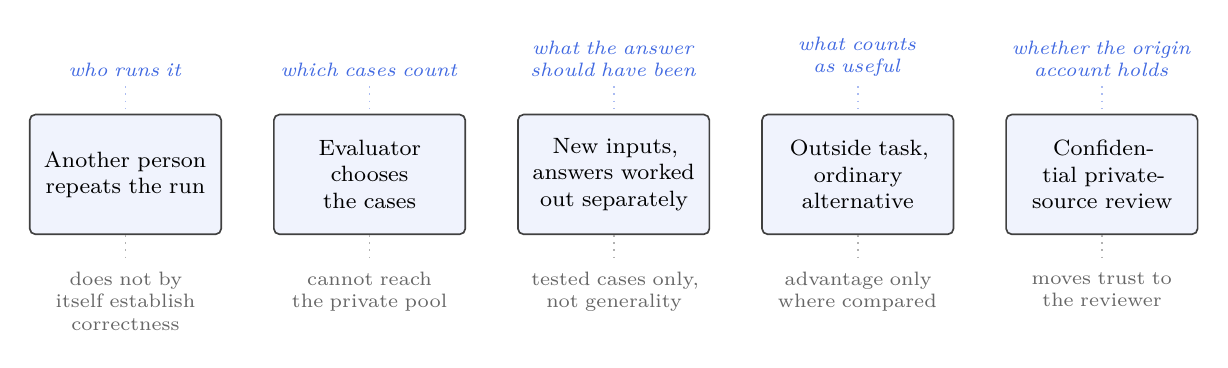
\begin{tikzpicture}[x=1cm,y=1cm]
% uniform box heights and bottom/top-anchored labels keep every dotted
% leader the same length
% a whisper of stranger-blue on the evaluations: each is evidence that lives
% outside the author's hands
\node[part, text width=2.15cm, minimum height=1.52cm, fill=strangerblue!8] (s1) at (1.2,0) {Another person repeats the run};
\node[part, text width=2.15cm, minimum height=1.52cm, fill=strangerblue!8] (s2) at (4.3,0) {Evaluator chooses the cases};
\node[part, text width=2.15cm, minimum height=1.52cm, fill=strangerblue!8] (s3) at (7.4,0) {New inputs, answers worked out separately};
\node[part, text width=2.15cm, minimum height=1.52cm, fill=strangerblue!8] (s4) at (10.5,0) {Outside task, ordinary alternative};
\node[part, text width=2.15cm, minimum height=1.52cm, fill=strangerblue!8] (s5) at (13.6,0) {Confidential private-source review};
\node[act, text width=2.25cm, anchor=south] (b1) at (1.2,1.12) {who runs it};
\node[act, text width=2.25cm, anchor=south] (b2) at (4.3,1.12) {which cases count};
\node[act, text width=2.25cm, anchor=south] (b3) at (7.4,1.12) {what the answer should have been};
\node[act, text width=2.25cm, anchor=south] (b4) at (10.5,1.12){what counts as useful};
\node[act, text width=2.25cm, anchor=south] (b5) at (13.6,1.12){whether the origin account holds};
\node[gnote, text width=2.25cm, anchor=north] (n1) at (1.2,-1.12){does not by itself establish correctness};
\node[gnote, text width=2.25cm, anchor=north] (n2) at (4.3,-1.12){cannot reach the private pool};
\node[gnote, text width=2.25cm, anchor=north] (n3) at (7.4,-1.12){tested cases only, not generality};
\node[gnote, text width=2.25cm, anchor=north] (n4) at (10.5,-1.12){advantage only where compared};
\node[gnote, text width=2.25cm, anchor=north] (n5) at (13.6,-1.12){moves trust to the reviewer};
\foreach \i in {1,...,5}{
  \draw[RoyalBlue!45, dotted, line width=0.6pt] (b\i.south) -- (s\i.north);
  \draw[black!30, dotted, line width=0.6pt] (s\i.south) -- (n\i.north);}
\end{tikzpicture}}
\caption{Five forms of independent evaluation. Above each evaluation, in italic
blue, the choice that leaves my hands; below it, in grey, what that evaluation
still cannot show. The evaluations are not cumulative stages. At the commit
this paper describes, the repository records none, and I know of none.}
\label{fig:ladder}
\end{figure}

\emph{Independent repetition} means a person with no involvement in the
project reruns the supplied commands in their own environment and publishes
what happened, including failures. That would reduce dependence on my
machine and test whether the published instructions suffice elsewhere. It
would not by itself establish correctness.

\emph{Evaluator-controlled selection} means the evaluator chooses
components from the full registry, without substitution when one proves
awkward, and original failures stay on the record even if I later repair
them. The units themselves are open to the same challenge: an evaluator
who finds that two entries are one dependent mechanism, or that a
boundary excludes the difficult part of a task, is disputing the registry,
not misusing it. That addresses curation within the public collection. It
cannot address whether the collection represents the private system,
because the private pool stays invisible.

\emph{Fresh inputs with independently derived expectations} can move
repeatability towards evidence bearing on correctness: inputs chosen after
the version is saved, and expected results worked out by a method that
does not pass through my code, whether independent calculation, a second
implementation, or an external reference. The result would support claims
about those cases only to the extent that the derivation is credible and
independent and the cases are adequate; general correctness still would not
follow.

\emph{Comparison on outside tasks} is what a claim of advantage over
ordinary alternatives would need: someone bringing a task that was not
designed around the project's own categories and comparing the component
against an ordinary alternative, which for several components would be a
short conventional script. Nothing in this paper makes that comparison.

\emph{A provenance review}, among the five evaluations shown here, bears most
directly on the origin story: a trusted person examining selected private
material against the public collection under confidentiality. Prior public
commitments could provide another kind of provenance evidence. Even
completed, this review would
transfer trust rather than remove it: public readers would be relying on
the reviewer's access, competence, and report instead of on mine, and the
review itself could not be published. The privacy cost may reasonably
never be paid. If it is not, the origin story remains testimony, and this
paper is written so that its argument does not depend on it.

\subsection*{How the record should age}

The evaluations above may expose failures. Repairs should add facts, not erase
them. The appendix keeps three failures at the pinned commit although a later
commit repairs one; that repair does not subtract the first fact. If criticism
shows a validator too weak or a claim too broad, record the revision's date and
cause instead of making the project appear always to have meant the narrower
claim. A test rewritten after its outcome is known is a different test and may
be better. The known case can show whether the same failure returns; fresh
confirmation requires new cases whose answers were not used to design the
repair. Disappointment is in scope: if an evaluation finds a component trivial
or no better than a short ordinary script, that conclusion belongs on the
record with the same standing as a pass. Any outside evaluator's report should
remain under that evaluator's control, cited rather than absorbed. If the
repository later falls short of this paragraph, the shortfall is itself a
finding, and Section~\ref{sec:conclusion} says where findings go.

These evaluations do not pair one-for-one with the distinctions. They address
the runner, public-case selection, tested-case correctness, usefulness, and origin.
None repairs a validator--claim mismatch, proves representativeness, or turns
risk reduction into a guarantee.

\section{Conclusion}
\label{sec:conclusion}

Plectis does not make the private system answerable as a whole. It publishes
fixed cases, procedures, outputs, rules, and limits so particular claims can
be challenged. A pass is no stronger than its rule or the expected answer's
basis.

More author-controlled components enlarge the inventory without changing who
chose the cases or rules. Moving a relevant choice out
of the author's hands can strengthen evidence about that choice; it does not
repair every gap.

\paragraph{A first review.} Use the appendix's no-install block and select the
version analysed here. The tour describes the checkout but does not choose a
component claim. Ask the repository to find the audio example with
\par\noindent\resizebox{\linewidth}{!}{\Verb|PYTHONPATH=src python3 -m plectis comprehend --first-action "audio level calculation" --format text|}\par
The response identifies the audio component, but do not run its first suggested
command: it writes to the repository's saved receipt paths. Run the paper's exact
no-install command near the start of Section~\ref{sec:run} instead; it writes only
to \code{/tmp} and leaves the checkout unchanged. Under
\component{/tmp/plectis-audio-rms/}, open
\component{batch8_audio_level_rms_port_result.json};
JSON is a plain-text field-and-value format. Open \code{exercise}. In each
\component{reference_cases} item, compare \code{expected\_level} with
\code{observed\_level}. The top-level \component{anti_claim} says what a pass
does not establish; \component{claim_ceiling} inside \code{exercise} gives the
project's strongest conclusion. The project wrote both cautions; no independent
reviewer checked their limits. To challenge rather than repeat the supplied case,
make a disposable copy of the fixture input:
\begin{Verbatim}[fontsize=\scriptsize]
cp -R fixtures/first_wave/batch8_audio_level_rms_port/input/. /tmp/plectis-audio-rms-input
\end{Verbatim}
In the copied \component{batch8_audio_level_rms_port_probe_manifest.json},
change the first case's second sample from \code{0.05} to \code{0.06}, but
leave \code{expected\_level} unchanged. Then run:
\begin{Verbatim}[fontsize=\scriptsize]
PYTHONPATH=src python3 -m plectis batch8-audio-level-rms-port run \
  --input /tmp/plectis-audio-rms-input --out /tmp/plectis-audio-rms-probe \
  --acceptance-out /tmp/plectis-audio-rms-check.json; echo $?
\end{Verbatim}
The final number printed should be \code{1}; in the acceptance file,
\code{status} should be \code{blocked} and \code{accepted} should be
\code{false}. This means the validator caught the deliberate mismatch; the
exercise did not crash. Report any different result in
\code{CONTRIBUTING.md}. Treat a pass as evidence only for the published rule.

\appendix
\small
\setlength{\parskip}{0pt}

\section{Dated reproduction record}
\label{sec:appendix}

Except where a paragraph gives a later date, this appendix records one run on
17~July~2026 under macOS 15.6.1 on Apple silicon (arm64) and Python 3.13.7.
The repository version was commit \code{\snapshotcommit}, abbreviated
\code{\snapshotshort} elsewhere. Later commits or machines may differ; the body
does not depend on them.

\paragraph{Names.} Repository: \repo. Formerly Microcosm, Plectis retains
package \code{microcosm\_core}, page \code{ORGANS.md} (``organs'' means
components), and the \code{microcosm} alias. This paper uses command
\code{plectis}.

\paragraph{Getting the code and running without installing.}

\begin{Verbatim}[fontsize=\small]
git clone https://github.com/wcook04/plectis
cd plectis
git checkout 57ffb7f5830c
PYTHONPATH=src python3 -m plectis tour --format text .
\end{Verbatim}

The final full stop means ``the current folder''. \code{git checkout} pins the
exact state described here; omit it to run the newest version, whose dated
numbers may differ.

The clean-clone tour read 5{,}018 files and chose the README-first order
(internally \component{readme_onboarding_route}) from five reading orders. It
wrote 21 generated files under \code{.microcosm/} without changing the examined
source. Those files can be rebuilt; the README's different count is another
dated run, not a stable project size.

\paragraph{Installing.}

\begin{Verbatim}[fontsize=\small]
python3 -m pip install .
plectis tour --format text .
\end{Verbatim}

No runtime library is required; \code{pip} may fetch \code{setuptools} to
build. No check proves the absence of network or model calls, so inspect the
source.

\paragraph{The worked example.} A fresh Section~\ref{sec:run} rerun reproduced
all displayed passes and values and overwrote \component{/tmp/plectis-audio-rms}.
A stale field reports a copied private module, while the saved import record
reports none because public code replaced it; the discrepancy remains.

\paragraph{A second Python version.} On 18~July~2026, a clean macOS clone under
Python 3.12.7 matched the tour and example. Its offline install used only the
machine's \code{setuptools} 80.9.0 (minimum 77.0.3). Only versions 3.12.7 and
3.13.7 were tested.

\paragraph{Project-wide checks.} The project-wide Lean trust scan checks
\leanfilecount{} files for six text patterns but does not run Lean or verify
proofs: unfinished placeholders; custom axioms
(unproved assumptions); compiled calculations whose acceptance
relies on more than Lean's small proof-checking core;
\code{partial} definitions (runnable but not unfoldable in proofs);
\code{unsafe} definitions (barred from theorems); and removed computation
limits. No pattern appeared. The scan does not show whether files compile,
proofs are valid, or statements express their authors' intent
\cite{leanvalidation}.
Separate components run Lean on small test projects; their results apply only
to those projects.
Registry and trust checks passed; the \leanfilecount{} files are distinct from
the \mathcount{} mathematics components.
The limited \code{make test} run covered 32 public test files, not every test
file: 356 of 361 tests passed, two skipped, and three failed. The
failures were an \code{AGENTS.md} line-break expectation; outdated line or byte
counts in copied-source manifests; and root-layout rules that did not yet allow
the \code{paper} directory or root PDF; the last was later repaired without
altering this pinned run. Exact failure names, environment, and counts are in
\component{paper/public-test-receipt.json}. \code{make ci} would add smoke and
package-install checks, but was not green because \code{make test} failed. These
checks cover only the public checkout; this is my run, not an independent
repetition.
The paper's own
\component{scripts/check_public_system_paper.py} fails if counts, pinned facts,
the example, cautions, or citations disagree. It checks historical facts against
the pinned commit separately from current prose; with one maintainer, that is
internal consistency, not external truth.

\begin{thebibliography}{10}
\fontsize{7.5pt}{8.3pt}\selectfont
\raggedright
\setlength{\itemsep}{0pt}
\setlength{\parsep}{0pt}
\setlength{\parskip}{0pt}

\bibitem{runeson2009}
Per Runeson and Martin H\"ost. ``Guidelines for Conducting and Reporting Case
Study Research in Software Engineering.'' \emph{Empirical Software
Engineering}, 14(2):131--164, 2009.
\href{https://doi.org/10.1007/s10664-008-9102-8}{doi:10.1007/s10664-008-9102-8}.

\bibitem{nasem2019}
National Academies of Sciences, Engineering, and Medicine.
\emph{Reproducibility and Replicability in Science}. Washington, DC:
The National Academies Press, 2019.
\href{https://doi.org/10.17226/25303}{doi:10.17226/25303}.

\bibitem{barr2015}
Earl T. Barr, Mark Harman, Phil McMinn, Muzammil Shahbaz, and Shin Yoo.
``The Oracle Problem in Software Testing: A Survey.''
\emph{IEEE Transactions on Software Engineering}, 41(5):507--525, 2015.
\href{https://doi.org/10.1109/TSE.2014.2372785}{doi:10.1109/TSE.2014.2372785}.

\bibitem{rosenthal1979}
Robert Rosenthal. ``The File Drawer Problem and Tolerance for Null Results.''
\emph{Psychological Bulletin}, 86(3):638--641, 1979.
\href{https://doi.org/10.1037/0033-2909.86.3.638}{doi:10.1037/0033-2909.86.3.638}.

\bibitem{omgsacm2023}
Object Management Group.
\href{https://www.omg.org/spec/SACM/2.3/PDF}{\emph{Structured Assurance Case Metamodel (SACM)}},
2.3, formal/23-05-08, October 2023.

\bibitem{acmartifact}
Association for Computing Machinery.
\href{https://www.acm.org/publications/policies/artifact-review-and-badging-current}{``Artifact Review and Badging---Current,''}
v1.1, 24 Aug. 2020; accessed 18 July 2026.

\bibitem{nistfips1804}
National Institute of Standards and Technology. \emph{Secure Hash Standard},
FIPS PUB 180-4, 2015.
\href{https://doi.org/10.6028/NIST.FIPS.180-4}{NIST FIPS 180-4}.

\bibitem{nisthashfunctions}
National Institute of Standards and Technology.
\href{https://csrc.nist.gov/projects/hash-functions}{``Hash Functions.''}
Updated 9 September 2024. Accessed 18 July 2026.

\bibitem{nasa8739}
National Aeronautics and Space Administration.
\emph{Software Assurance and Software Safety Standard},
NASA-STD-8739.8B, Section 4.4.1.2, 2022.
\href{https://standards.nasa.gov/standard/NASA/NASA-STD-87398}{NASA-STD-8739.8B}.

\bibitem{leanvalidation}
Lean Project. \emph{Lean Language Reference} sections
\href{https://lean-lang.org/doc/reference/latest/ValidatingProofs/}{``Validating a Lean Proof''} and
\href{https://lean-lang.org/doc/reference/latest/Definitions/Recursive-Definitions/#partial-and-unsafe-definitions}{``Partial and Unsafe Definitions.''}
Accessed 18 July 2026.

\end{thebibliography}

\end{document}
